
\section{圆}

\section{三角形}

\section{尺规作图}

尺规作图(ruler-and-compass construction)使用无刻度的直尺和圆规作出给定图形。允许的操作包括: 过两已知点作直线（计为一步）；以已知点为圆心过已知点作圆（计为一步）；取位于至多两个直线或圆上的一个点（不计步数）。

\begin{pro}\textbf{以给定长度为半径作圆}(步数5)
\par 如图\ref{fig:plg_rc_compass}, 给定线段AB和点C, 以C为圆心、AC为半径作圆$R_1$；分别以A为圆心、AB、AC为半径作圆$R_2$, $R_3$. $R_1$交$R_2$于点D, 交$R_3$于点E. 以E为圆心、DE为半径作圆，交$R_3$于点F, 则$CF=AB$. 
\end{pro}
\begin{proof}
易得$\triangle AEF \cong \triangle CED$, 故$\angle AED = \angle CEF$, 进而$\triangle AED \cong \triangle CEF$, 得证. 
\end{proof}

\begin{figure}[htb]
\centering
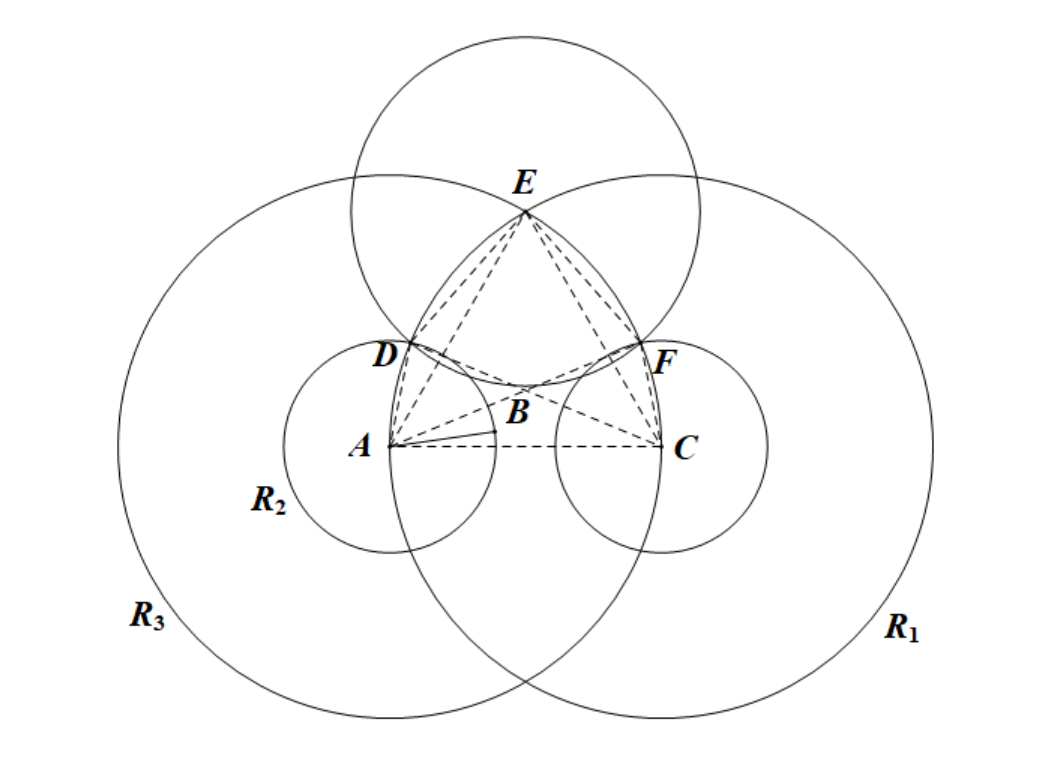
\includegraphics[width=10cm]{fig/plg_rc_compass.png}
\caption{以给定长度为半径作圆}
\label{fig:plg_rc_compass}
\end{figure}

上述命题表明尺规作图的作圆操作等价于“以已知点为圆心，两已知点距离为半径作圆”. 一种更为简明的作法是: 不妨设A、B、C三点不共线, 过C作AB平行线, 过B作AC平行线, 两直线交于点F, 则$CF=AB$. 


\begin{pro}\textbf{作线段中垂线}(步数3)
\par 如图\ref{fig:plg_rc_midpoint}, 给定线段AB, 以A为圆心、AB为半径作圆A，以B为圆心、AB为半径作圆B，两圆交于C、D，作直线CD交线段AB于M, 则$AM=BM$, 且$CD\perp AB$. 
\end{pro}
\begin{proof}
易得$\triangle ADC \cong \triangle BDC$, 故$\angle ACM = \angle BCM$. 又由$AC=BC$, $\triangle ACM \cong \triangle BCM$. 故$AM=BM$, $\angle AMC=\angle BMC=\frac{\pi}{2}$.
\end{proof}

\begin{pro}\textbf{作角平分线}(步数4)
\par 如图\ref{fig:plg_rc_bisectangle}, 以A为圆心的圆交角的两边于B, C；以B为圆心、BC为半径作圆，以C为圆心、BC为半径作圆，两圆交于D, 则$\angle BAD = \angle CAD$. 
\end{pro}

\begin{figure}[h]
\begin{minipage}{0.48\textwidth}
\centering
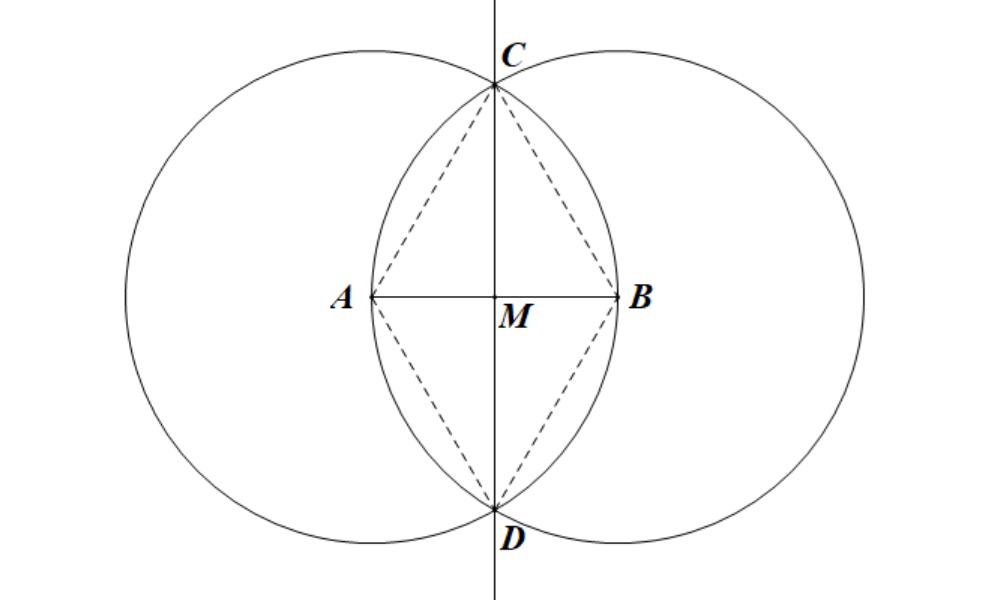
\includegraphics[width=7.5cm]{fig/plg_rc_midpoint.png}
\caption{尺规作线段中垂线}
\label{fig:plg_rc_midpoint}
\end{minipage}\hfill
\begin{minipage}{0.48\textwidth}
\centering
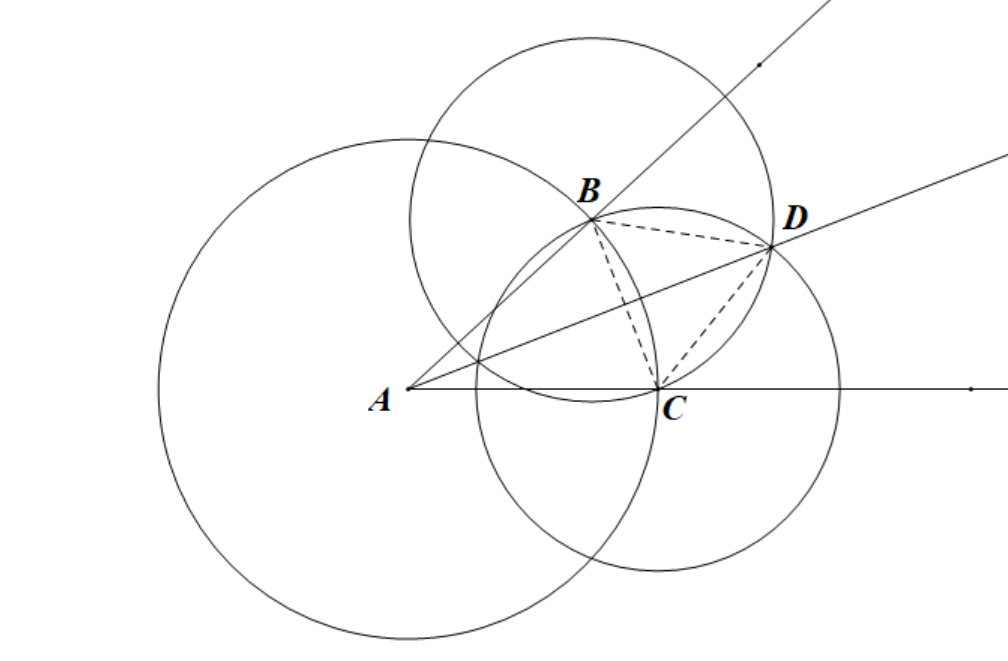
\includegraphics[width=7.5cm]{fig/plg_rc_bisectangle.png}
\caption{尺规作角平分线}
\label{fig:plg_rc_bisectangle}
\end{minipage}
\end{figure}


\begin{pro}\textbf{过直线外一点作垂线}(步数3)
\par 如图\ref{fig:plg_rc_perpendicular1}, 给定直线BC外一点A，以B为圆心、AB为半径作圆，以C为圆心、AB为半径作圆，两圆交于D, 则$AD \perp BC$. 
\end{pro}

\begin{pro}\textbf{过直线上一点作垂线}(步数3)
\par 如图\ref{fig:plg_rc_perpendicular2}, 给定直线上一点A，任取直线外一点O, 以O为圆心、OA为半径作圆，交直线于另一点B; 直线BO交圆O于点C, 则$CA \perp AB$. 
\end{pro}

\begin{figure}[h]
\begin{minipage}{0.48\textwidth}
\centering
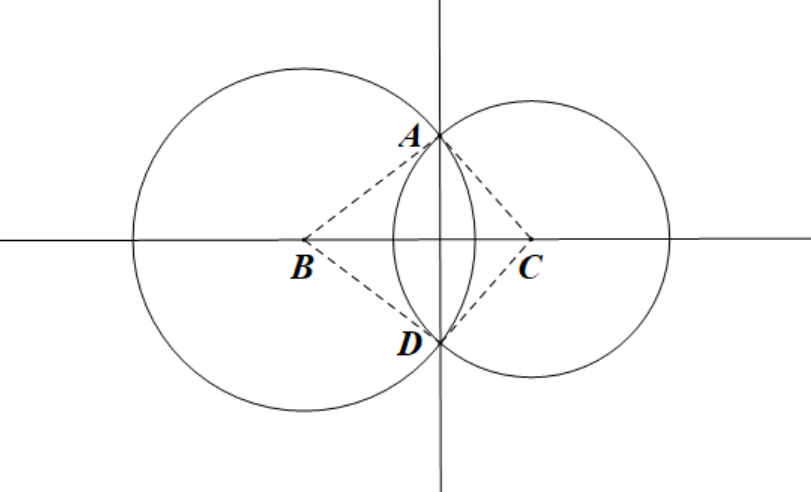
\includegraphics[width=8cm]{fig/plg_rc_perpendicular1.png}
\caption{尺规作过直线外一点的垂线}
\label{fig:plg_rc_perpendicular1}
\end{minipage}\hfill
\begin{minipage}{0.48\textwidth}
\centering
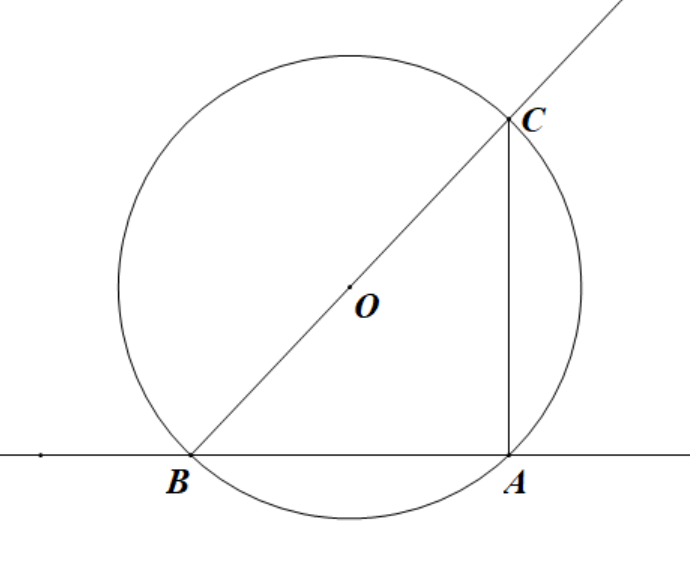
\includegraphics[width=6cm]{fig/plg_rc_perpendicular2.png}
\caption{尺规作过直线上一点的垂线}
\label{fig:plg_rc_perpendicular2}
\end{minipage}\hfill
\end{figure}

\begin{pro}\textbf{过直线外一点作平行线}(步数4)
\par 如图\ref{fig:plg_rc_parallel}, 给定直线AB外一点C，以A为圆心、AC为半径作圆，以B为圆心、BC为半径作圆，两圆交于C、D. 连接BD交圆B于点E, 则$CE \parallel AB$.  
\end{pro}

\begin{figure}[htb]
\centering
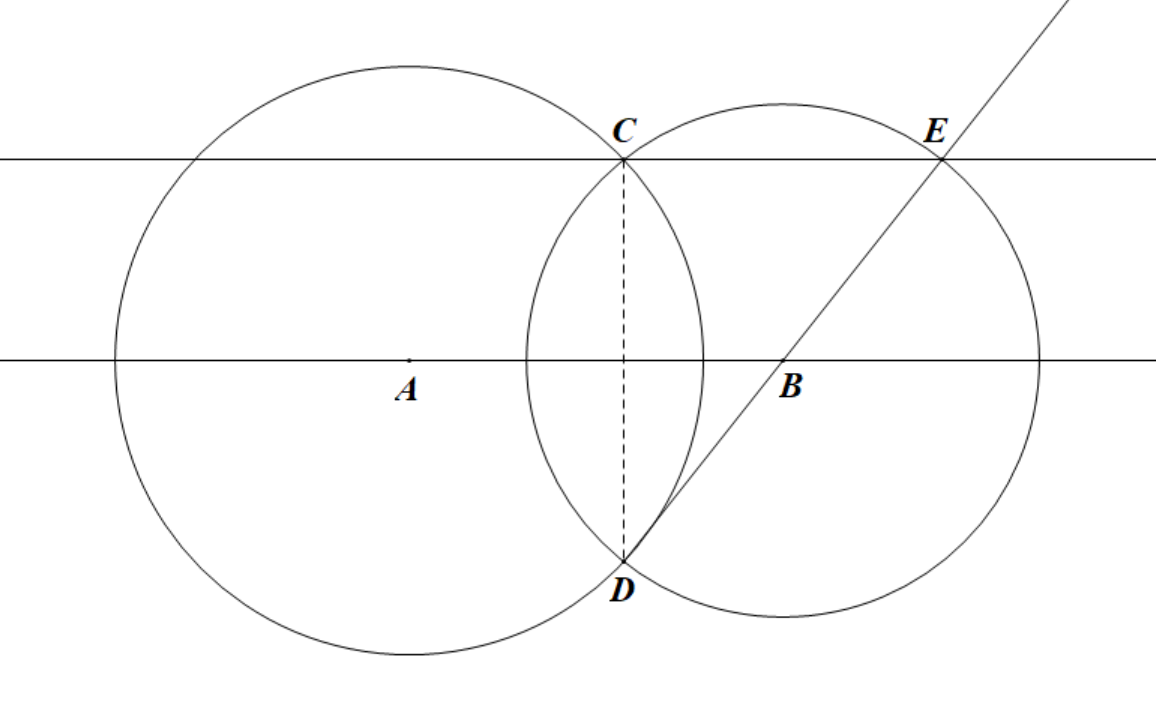
\includegraphics[width=8cm]{fig/plg_rc_parallel.png}
\caption{过直线外一点作平行线}
\label{fig:plg_rc_parallel}
\end{figure}

\section*{阅读材料}

互动游戏Euclidea\cite{Euclidea}包含大量尺规作图问题，许多问题最少步数的作法很具挑战性。

\section*{问题}
\newcounter{probplg} 

\stepcounter{probplg}
\par \textbf{\theprobplg .} \textbf{(作角等于已知角)} 给定$\angle A$和射线BC, 用尺规作$\angle DBC = \angle A$. 

\stepcounter{probplg}
\par \textbf{\theprobplg .} \textbf{(尺规作图的限度)} 设$z_1,z_2\in \mathbb{C}$, $r$是非负实数, 记$L(z_1,z_2)=\{z\in \mathbb{C}\vert \exists t\in \mathbb{R}: z=z_1+t(z_2-z_1)\}$; $C(z_1,r)=\{z\in \mathbb{C} : |z-z_1|=r\}$. 定义$\mathcal{P}_0=\{0,1\}$, $\mathcal{L}_0=\mathcal{C}_0=\varnothing$, 
\begin{align*}
\mathcal{L}_{n+1} & = \{L(z_1,z_2)\vert z_1, z_2\in \mathcal{P}_n \land z_1\neq z_2\}\\
\mathcal{C}_{n+1} & = \{C(z_1,|z_2-z_3|)\vert z_1, z_2, z_3\in \mathcal{P}_n \land  z_2\neq z_3\}\\
\mathcal{P}_{n+1} &  = \{z\in \mathbb{C} \vert \exists L_1,L_2\in \mathcal{L}_{n+1}: L_1 \neq L_2 \land z\in L_1\cap L_2\}\\
& \cup \{z\in \mathbb{C} \vert \exists C_1,C_2\in \mathcal{C}_{n+1}: C_1 \neq C_2 \land z\in C_1\cap C_2\} \\
&  \cup \{z\in \mathbb{C} \vert \exists C\in \mathcal{C}_{n+1} \exists L\in \mathcal{L}_{n+1}: z\in C\cap L\}
\end{align*}
并记$\mathcal{P}=\bigcup_{n\in \mathbb{N}} \mathcal{P}_{n}$. 

设$z\in \mathbb{C}$, 若存在$n\in\mathbb{N}$以及$\mathbb{C}$的子域$K_1,\dots,K_n$, 满足
\begin{equation*}
    \mathbb{Q}=K_0\subseteq K_1 \subseteq \cdots \subseteq K_n
\end{equation*}
$z\in K_n$, 且$[K_j:K_{j-1}]\le 2$对任意$j=1,\dots,n$成立, 称$z$为可构造数. 可构造数的集合记为$\mathbb{Q}^c$. 

设$\mathbb{C}$的子域$K$满足$z\in K \Rightarrow \exists r\in K: r^2=z$, 称$K$对开平方封闭. 

证明: 
(1) $\forall n\in \mathbb{N}$,  $\mathcal{P}_{n}$是有限集. 
(2) $\forall n\in \mathbb{N}$,  $\mathcal{P}_{n}\subseteq \mathcal{P}_{n+1}$. 
(3) $\forall n\in \mathbb{N}$, $z\in \mathcal{P}_n \Rightarrow \bar{z}\in \mathcal{P}_n$.
(4) $\mathbb{Q}^c$是$\mathbb{C}$的子域. 
(5) $z\in \mathbb{Q}^c \Rightarrow \bar{z} \in \mathbb{Q}^c$. 
(6) $\mathbb{Q}^c$对开平方封闭. 设$\mathbb{C}$的子域$K$对开平方封闭, 则$\mathbb{Q}^c \subseteq K$. 
(7) $z,w\in \mathcal{P} \Rightarrow z+w, -z, zw \in \mathcal{P}$; 当$z\neq 0$, 亦有$z^{-1}\in \mathcal{P}$. $\mathcal{P}$对开平方封闭.
(8) $\mathcal{P}=\mathbb{Q}^c$.
(9*) $\alpha\in \mathcal{P} \Rightarrow \exists k\in \mathbb{N}:[\mathbb{Q}(\alpha): \mathbb{Q}] = 2^k$. 举例说明逆命题不成立. 
(10) (\textbf{倍立方问题}) $\sqrt[3]{2}\notin \mathcal{P}$. 
(11) (\textbf{化圆为方问题}) $\sqrt{\pi}\notin \mathcal{P}$.
(12) (\textbf{三等分角问题}) $e^{\frac{2\pi \mathrm{i}}{3}}\in \mathcal{P}$, $e^{\frac{2\pi \mathrm{i}}{9}}\notin \mathcal{P}$.

\stepcounter{probplg}
\par \textbf{\theprobplg .} \textbf{(尺规作正多边形的可行性)}

(1*) 设$p$是素数, 则正$p$边形可用尺规作出当且仅当存在$k\in\mathbb{N}$, $p= 2^{2^k}+1$, 即$p$是Fermat素数. 

\stepcounter{probplg}
\par \textbf{\theprobplg .} \textbf{(有刻度直尺三等分角)} 如图\ref{fig:plg_trisect_angle}, 给定$\angle AOB$, 其中$A,B$位于以$O$为圆心、$r$为半径的圆上. 过$A$的直线交圆$O$于$D$, 交直线$BO$于$C$, 满足$CD=r$. 证明: $\angle ACB = \frac{1}{3} \angle AOB$. 

\begin{figure}[h]
\centering
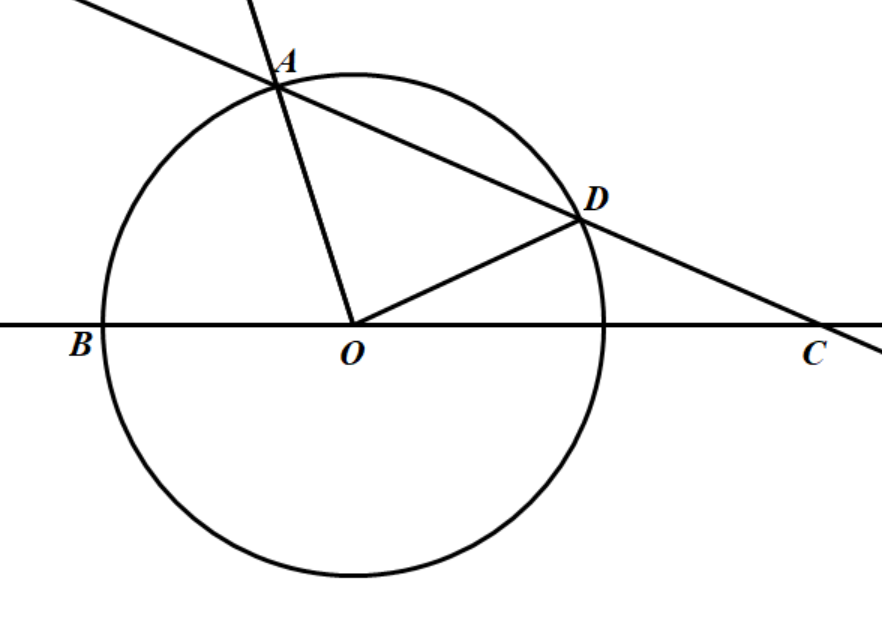
\includegraphics[width=6cm]{fig/plg_trisection_angle.png}
\caption{有刻度直尺三等分角}
\label{fig:plg_trisect_angle}
\end{figure}

\section*{解答}
\newcounter{solplg} 

\stepcounter{solplg}
\par \textbf{\thesolplg .} 如图\ref{fig:plg_copyangle}, 以任意长为半径作圆A交角的两边于E、F; 以B为圆心、AE为半径作圆交射线BC于G；以G为圆心、EF为半径作圆交圆B于D，则$\angle DBC = \angle A$. 

\begin{figure}[h]
\centering
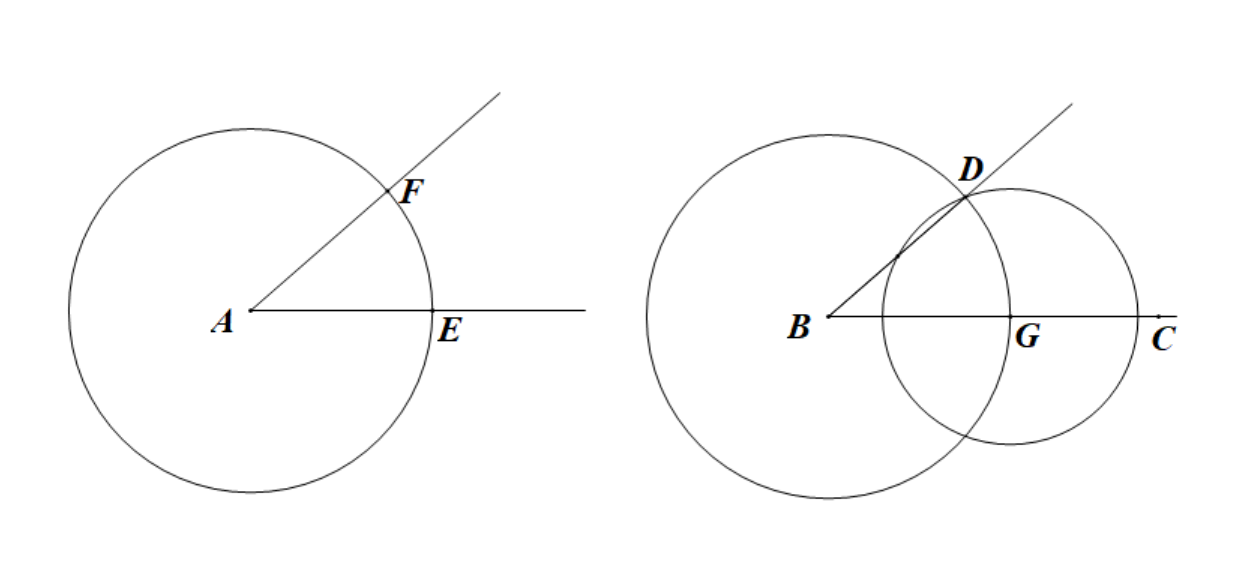
\includegraphics[width=9.6cm]{fig/plg_rc_copyangle.png}
\caption{作角等于已知角}
\label{fig:plg_copyangle}
\end{figure}

\stepcounter{solplg}
\par \textbf{\thesolplg .} (1) 对$n$归纳证明$\mathcal{L}_n$, $\mathcal{C}_n$, $\mathcal{P}_n$都是有限集. (2) 对$n$归纳证明$\mathcal{L}_n\subseteq \mathcal{L}_{n+1}$, $\mathcal{C}_n\subseteq \mathcal{C}_{n+1}$, $\mathcal{P}_n\subseteq \mathcal{P}_{n+1}$. 

(3) 对$n$归纳. $n=0$时显然成立. 设命题对$n-1$成立, 则$L(z_1,z_2)\in \mathcal{L}_n \Rightarrow L(\bar{z}_1,\bar{z}_2)\in \mathcal{L}_n$, $C(z_1,|z_2-z_3|)\in \mathcal{C}_n \Rightarrow C(\bar{z}_1,|\bar{z}_2-\bar{z}_3|)\in \mathcal{C}_n$. 当$z\in \mathcal{P}_n$, $z$为$\mathcal{P}_{n-1}$中特定点确定的$\mathcal{L}_n$中直线和/或$\mathcal{C}_n$中圆的交点，$\bar{z}$为其共轭点确定的$\mathcal{L}_n$中直线和/或$\mathcal{C}_n$中圆的交点，故$\bar{z}\in \mathcal{P}_n$. 

(4) 对$x,y\in \mathbb{Q}^c$, 设$\mathbb{C}$的子域$K_1,\dots,K_n$; $L_1,\dots, L_m$满足
\begin{align*}
\mathbb{Q}&=K_0 \subseteq K_1 \subseteq \cdots \subseteq K_n\\
\mathbb{Q}&=L_0 \subseteq L_1 \subseteq \cdots \subseteq L_m
\end{align*}
且$[K_i:K_{i-1}]=2$, $i=1,\dots,n$; $[L_j:L_{j-1}]=2$, $j=1,\dots,m$; $x\in K_n$, $y\in L_m$. 由素数次扩张是单扩张, 可设$K_i=K_{i-1}(\alpha_i)$, $i=1,\dots,n$; $L_j=L_{j-1}(\beta_j)$, $j=1,\dots,m$. 对$j=1,\dots,m$, 令$K_{n+j}=K_{n+j-1}(\beta_j)$, 则$x,y\in K_{n+m}$. 对$j=1,\dots,m$, 由于$\beta_j$在$L_{j-1}$上的极小多项式次数为2, 而$L_{j-1} \subseteq K_{n+j-1}$, 因此$\beta_j$在$K_{n+j-1}$上的极小多项式次数至多为2, $[K_{n+j},K_{n+j-1}]\le 2$. 因此$K_{n+m}$中的元素都是可构造数, 从而$x-y, xy$是可构造数; 当$y\neq 0$, $y^{-1}$也是可构造数. 命题得证. 

(5) 设$\mathbb{C}$的子域$K_1,\dots,K_n$满足$\mathbb{Q}=K_0 \subseteq K_1 \subseteq \cdots \subseteq K_n$, $z\in K_n$, 且$[K_i:K_{i-1}]=2$, $i=1,\dots,n$. 因此有$\mathbb{Q}=K_0 \subseteq \bar{K}_1 \subseteq \cdots \subseteq \bar{K}_n$, $\bar{z}\in \bar{K}_n$, 其中$\bar{K}_i = \{\bar{x} \vert x\in K_i\}$. 由$K_i$为$\mathbb{C}$的子域, $\bar{K}_i$也为$\mathbb{C}$的子域. 事实上, 设$x,y \in \bar{K}_i$, 则$\bar{x},\bar{y}\in K_i$, $\overline{x-y}=\bar{x}-\bar{y} \in K_i$, $\overline{xy}=\bar{x}\bar{y} \in K_i$; 从而$x-y, xy\in \bar{K}_i$. 当$y\neq 0$, $0 \neq \bar{y}\in K_i$, $\overline{y^{-1}}=(\bar{y})^{-1}\in K_i$, $y^{-1}\in \bar{K}_i$. 最后证明$[\bar{K}_i:\bar{K}_{i-1}]=[K_i:K_{i-1}]=2$. 事实上, 设$z_{i,1},z_{i,2}$是$K_{i-1}$上线性空间$K_i$的一个基, 则$\bar{z}_{i,1},\bar{z}_{i,2}$是$\bar{K}_{i-1}$上线性空间$\bar{K}_i$的一个基. 

(6) 设$z\in \mathbb{Q}^c$，则存在$\mathbb{C}$的子域$K_1,\dots,K_n$满足$\mathbb{Q}=K_0 \subseteq K_1 \subseteq \cdots \subseteq K_n$, $z\in K_n$, 且$[K_i:K_{i-1}]=2$, $i=1,\dots,n$. 设$r\in \mathbb{C}$是$x^2 - z$的一个零点, 令$K_{n+1}=K_n (r)$，则$[K_{n+1}: K_n] \le 2$, 故$r\in \mathbb{Q}^c$. 

设$\mathbb{C}$的子域$K$对开平方封闭, 对$n$归纳证明: 若$\mathbb{C}$的子域$K_1,\dots,K_n$满足$\mathbb{Q}=K_0 \subseteq K_1 \subseteq \cdots \subseteq K_n$, $z\in K_n$, 且$[K_i:K_{i-1}]=2$, $i=1,\dots,n$, 则$K_n \subseteq K$. 当$n=0$时, $\mathbb{Q}\subseteq K$显然成立. 设命题对$n-1$成立, 由素数次扩张是单扩张, 可设$K_n=K_{n-1}(\alpha)$. 设$\alpha$在$K_{n-1}$上的极小多项式为$x^2 + bx + c$, $b,c \in K_{n-1} \subseteq K$, 则由一元二次方程的求根公式及$K$对开平方封闭, 知$\alpha\in K$. 因此$K_n \subseteq K$. 得证.

(7) 命题即证明从给定复数出发, 由四则及开平方运算得到的复数对应的点可由尺规作出. 
\par (i) 设$\overrightarrow{OA}=z$， $\overrightarrow{OB}=w$, 当$O, A, B$不共线时，过A作OB的平行线，过B作OA的平行线，两直线交于$C$, 则$\overrightarrow{OC}=z+w$. 当$O, A, B$共线时，$C(z,|w|)$与$L(0,z)$的交点之一即为$z+w$. 
\par (ii) $C(0,|z|)$与$L(0,z)$的另一个交点即为$-z$. 
\par (iii) 为作$zw$, 只需作出角度$\arg z+\arg w$和长度$|z|\cdot |w|$. 前者只需以OA为一边向逆时针方向作角等于$\arg w$. 为作长度$|z|\cdot |w|$, 不妨设$z,w\neq 0$. 如图\ref{fig:plg_segmentmul}, 设$\overrightarrow{OA}=|z|$， $\overrightarrow{OB}=|w|$, $\overrightarrow{OC}=1$, 作$\overrightarrow{OD}=i$, $\overrightarrow{OE}=i|z|$, 过E作BD的平行线交OC于F, 则 $\overrightarrow{OF}=|z||w|$.

\begin{figure}[h]
\begin{minipage}{0.5\textwidth}
\centering
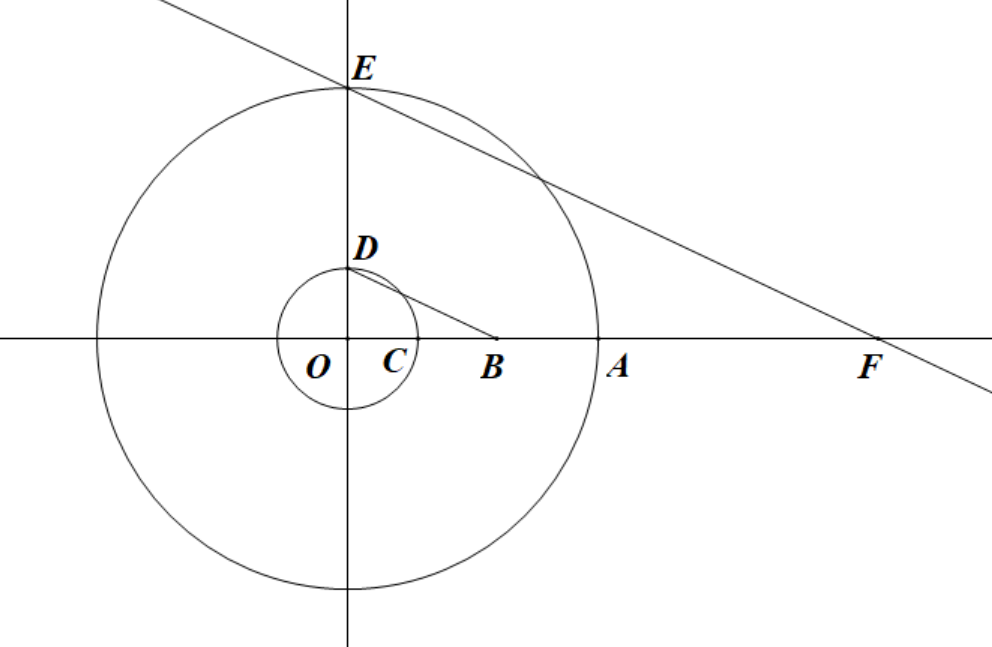
\includegraphics[width=7.2cm]{fig/plg_rc_segmentmul.png}
\caption{作线段长度乘积}
\label{fig:plg_segmentmul}
\end{minipage}\hfill
\begin{minipage}{0.5\textwidth}
\centering
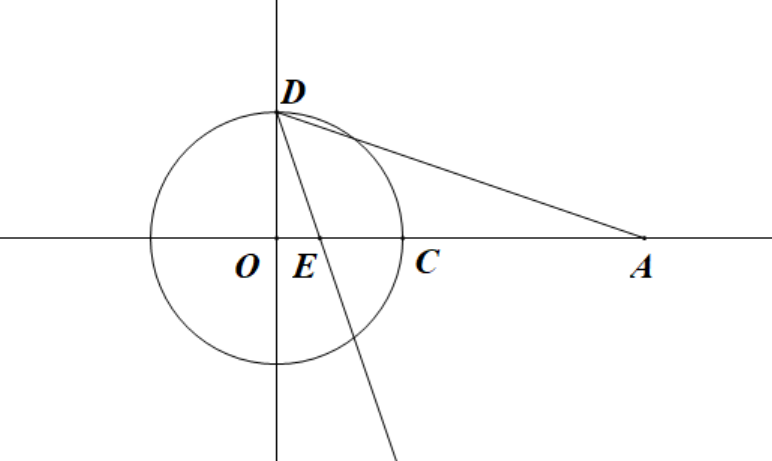
\includegraphics[width=7.2cm]{fig/plg_rc_segmentinv.png}
\caption{作线段长度倒数}
\label{fig:plg_segmentinv}
\end{minipage}\hfill
\end{figure}

\par (iv) 容易做出$\arg (z^{-1})=-\arg z$. 为作$|z^{-1}|=|z|^{-1}$, 设$\overrightarrow{OA} = |z|$, 如图\ref{fig:plg_segmentinv}, 设$\overrightarrow{OC}=1$, 作$\overrightarrow{OD}=i$, $\angle ODE = \angle OAD$, 则$OE = |z|^{-1}$. 

\par (v) 通过作角平分线容易做出$\arg \sqrt{z} = \frac{1}{2}\arg z$. 为作$|\sqrt{z}|=\sqrt{|z|}$, 不妨设$z\neq 0$, 如图\ref{fig:plg_segsqrt}, 设$\overrightarrow{OA}=|z|$, $\overrightarrow{OC}=1$, 容易作出$\overrightarrow{OD}=-1$. 作AD的中点E, $C(E, |DE|)$交纵轴于点F, 则$|OF|=\sqrt{|z|}$. 
由(ii)可作出$-\sqrt{z}$. 

\begin{figure}[h]
\centering
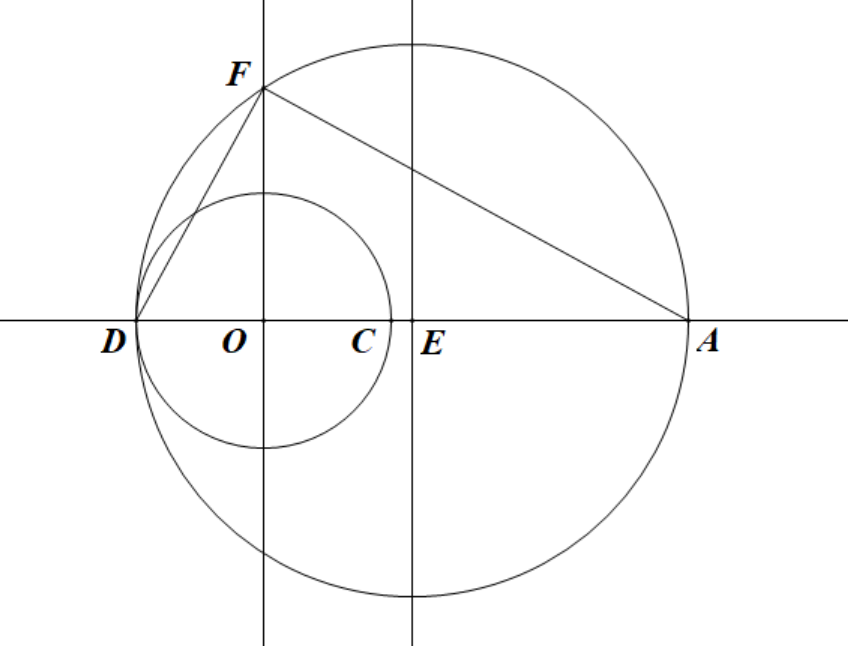
\includegraphics[width=8cm]{fig/plg_rc_segsqrt.png}
\caption{作线段长度平方根}
\label{fig:plg_segsqrt}
\end{figure}


(8) 先证$\mathcal{P} \subseteq \mathbb{Q}^c$. 对$n$归纳证明$\mathcal{P}_n \subseteq \mathbb{Q}^c$. $n=0$显然成立. 设命题对$n$成立, 考虑$n+1$的情形, 对$z\in \mathcal{P}_{n+1}$，分三种情况：(a) $z$是不同直线$L(z_1, z_2), L(z_3, z_4)$的交点, $z_1,z_2,z_3,z_4 \in \mathbb{Q}^c$. 由(5), 其共轭也属于$\mathbb{Q}^c$. 存在$a,b\in \mathbb{R}$, $z=az_1+(1-a)z_2=bz_3+(1-b)z_4$. 此时有
\begin{align*}
    (z_1-z_2)a+(z_4-z_3)b &= z_4-z_2\\
    (\bar{z}_1-\bar{z}_2)a+(\bar{z}_4-\bar{z}_3)b &= \bar{z}_4-\bar{z}_2
\end{align*}
上述关于$a,b$的线性方程组有唯一解，故$a$可由$z_1,z_2,z_3,z_4$及其共轭的加减乘除运算表出, $a\in \mathbb{Q}^c$, 从而$z\in \mathbb{Q}^c$. (b) $z$是直线$L(z_1, z_2)$与圆$C(z_3, |z_4-z_5|)$的交点, $z_1,z_2,z_3, z_4, z_5 \in \mathbb{Q}^c$. 令$r=|z_4-z_5|$, 则存在$a, \theta\in \mathbb{R}$, $z=az_1+(1-a)z_2=z_3+re^{\mathrm{i}\theta}$. 
此时有
\begin{align*}
    (z_1-z_2)a+z_2-z_3 &= re^{\mathrm{i}\theta}\\
    (\bar{z}_1-\bar{z}_2)a+\bar{z}_2-\bar{z}_3 &= re^{-\mathrm{i}\theta}
\end{align*}
两式相乘得
\begin{equation*}
    (a(z_1-z_2)+z_2-z_3)(a(\bar{z}_1-\bar{z}_2)+\bar{z}_2-\bar{z}_3) = r^2=(z_4-z_5)(\bar{z}_4-\bar{z}_5)
\end{equation*}
此为关于$a$的二次方程, 其系数均在$\mathbb{Q}^c$中. 由$\mathbb{Q}^c$对开平方封闭, $a\in \mathbb{Q}^c$, 从而$z\in \mathbb{Q}^c$. (c) $z$是不同圆$C(z_1, |z_2-z_3|)$与$C(z_4, |z_5-z_6|)$的交点, $z_1,z_2,z_3, z_4, z_5, z_6 \in \mathbb{Q}^c$. 令$r=|z_2-z_3|$, $s=|z_5-z_6|$, 则存在$\theta, \phi\in \mathbb{R}$, $z=z_1+re^{\mathrm{i}\theta}=z_4+se^{\mathrm{i}\phi}$.  
此时有
\begin{align*}
    (z-z_1)(\bar{z}-\bar{z}_1)&= r^2\\
    (z-z_4)(\bar{z}-\bar{z}_4)&= s^2
\end{align*}
消去$\bar{z}$得到关于$z$的二次方程, 其系数均在$\mathbb{Q}^c$中, 故$z\in \mathbb{Q}^c$.

\par 再证$\mathbb{Q}^c \subseteq \mathcal{P}$. 对$n$归纳证明: 若$\mathbb{C}$的子域$K_1,\dots,K_n$满足$\mathbb{Q}=K_0 \subseteq K_1 \subseteq \cdots \subseteq K_n$, 且$[K_i:K_{i-1}]=2$, $i=1,\dots,n$, 则$K_n \subseteq \mathcal{P}$. 由(7), 任意$q\in \mathbb{Q}$可由$0,1$出发用尺规作出, 从而$\mathbb{Q}\subseteq \mathcal{P}$, $n=0$成立. 设命题对$n$成立, 则由$[K_{n+1}:K_n]=2$知存在$\alpha\in K_{n+1}$, $K_{n+1} = K_n(\alpha)$, 且$\alpha$的极小多项式次数为2. 由二次方程求根公式, $\alpha$可由$K_n$中的数经过四则运算及开平方得到, 由$K_n \subseteq \mathcal{P}$及(7), $\alpha\in \mathcal{P}$, 从而$K_{n+1}\subseteq \mathcal{P}$. 得证. 

\emph{注}: 尺规作图的给定点可推广到有限集$P\subseteq \mathbb{C}$, 满足$\{0,1\} \subseteq P$, 且$z\in P\Rightarrow \bar{z} \in P$. 此时改为$\mathcal{P}_0=P$, 同理可证复数$z$可用尺规作出的充要条件为: 存在$n\in \mathbb{N}$及$\mathbb{C}$的子域$K_1,\dots,K_n$, 满足$\mathbb{Q}(P) = K_0 \subseteq K_1 \subseteq \cdots \subseteq K_n$, $z\in K_n$, $[K_j:K_{j-1}]\le 2$对任意$j=1,\dots,n$成立. 

(9) 由(8)及域扩张次数的性质即得. 

(10) 由Eisenstein判别法, $x^3-2$在$\mathbb{Q}[x]$上不可约, 因此$x^3-2$是$\sqrt[3]{2}$在$\mathbb{Q}$上的极小多项式, $[\mathbb{Q}(\sqrt[3]{2}): \mathbb{Q}]=3$. 

(11) 若$\sqrt{\pi}\in \mathcal{P}$, 则$\pi \in \mathcal{P}$. 但由Lindemann定理, $\pi$是$\mathbb{Q}$上的超越元, $[\mathbb{Q}(\pi):\mathbb{Q}]$无限, 矛盾. 

(12) 设$\zeta=e^{\frac{2\pi i}{9}}\in \mathcal{P}$, 则$\alpha = \zeta + \zeta^{-1} \in \mathcal{P}$. 而$\alpha^3 = \zeta^6 + \zeta^3 + 3\zeta + 3\zeta^{-1} = -1 + 3\alpha$, 因此$\alpha$是$x^3-3x+1$的一个零点. 容易验证$x^3-3x+1$在$\mathbb{Z}[x]$上不可约（$|x||x^2-3|=1$没有整数解），由Gauss引理，其在$\mathbb{Q}[x]$上也不可约, 从而是$\alpha$的极小多项式, $[\mathbb{Q}(\alpha):\mathbb{Q}]=3$, 矛盾. 

\stepcounter{solplg}
\par \textbf{\thesolplg .} 正$p$边形的外角为$\frac{2\pi}{p}$. 因此正$p$边形可用尺规作出等价于$\zeta_p=e^{\frac{2\pi i}{p}}$是可构造数. 必要性: $e^{\frac{2\pi i}{p}}$是$\Phi_p(z)=\frac{z^{p}-1}{z-1}=1+z+\cdots z^{p-1}$的一个零点. 当$p$为素数时, $\Phi_p(z)$在$\mathbb{Q}[x]$上不可约, 从而是$\zeta_p$在$\mathbb{Q}$上的极小多项式. 因此$[\mathbb{Q}(\zeta_p):\mathbb{Q}]=p-1$, 故存在正整数$m$, $p=2^m+1$. 若$m$包含奇素因子$b$, 设$m=ab$, 则$2^a+1\vert 2^{ab}+1$, 与$p$是素数矛盾. 故$m$只能为2的非负整数次幂, 即$p$是Fermat素数. 

\stepcounter{solplg}
\par \textbf{\thesolplg .} $\angle AOB=\angle OAD +\angle ACB$. 由$OA=OD=CD$, $\angle OAD = \angle ODA = 2\angle ACB$.  